\documentclass[11pt]{article}
\usepackage[margin=1in]{geometry}
\usepackage{array}
\usepackage{booktabs}
\usepackage{enumitem}
\usepackage{float}
\usepackage{graphicx}
\usepackage{hyperref}
\usepackage{longtable}
\setlength{\parindent}{0pt}
\setlength{\parskip}{0.6em}

\title{Unified Prompt-Profile Report:\\Setup, Views, Results, and Mechanism}
\author{}
\date{2026-04-09 22:55 UTC}

\begin{document}
\maketitle

\section*{Executive Summary}
\begin{itemize}[leftmargin=1.5em]
\item This is the single current prompt-profile report surface.
  \begin{itemize}[leftmargin=1.5em]
  \item Regression stays on the natural prompt-disjoint split with natural sampling.
  \item Classification stays on balanced train with natural test.
  \item The same note now carries setup, predictor views, metrics, results, and the plain-English metadata explanation in one place.
  \end{itemize}
\item Regression read:
  \begin{itemize}[leftmargin=1.5em]
  \item \texttt{mean\_relative\_length} is useful as a screening score, not as a clean calibrated regressor.
  \item On \texttt{top\_20p\_capture}, ensemble beats prompt length on \texttt{GPQA}, \texttt{MMLU-Pro}, and \texttt{LiveCodeBench}.
  \end{itemize}
\item Classification read:
  \begin{itemize}[leftmargin=1.5em]
  \item \texttt{majority\_s\_0.5} is still the cleaner deployment-facing head.
  \item The best single global activation surface is still \texttt{ensemble h256 d1}.
  \end{itemize}
\item Metadata read:
  \begin{itemize}[leftmargin=1.5em]
  \item The old reported metadata baseline is only prompt length on this fixed-budget run.
  \item Prompt-only cues are strong mostly because prompt surface structure already carries much of the same long-completion signal.
  \item \texttt{GPQA} is the main exception where raw length is weak and prompt structure matters more.
  \end{itemize}
\end{itemize}

\section*{Setup}
\subsection*{Common rollout contract}
\begin{itemize}[leftmargin=1.5em]
\item model: \texttt{Qwen/Qwen3-1.7B}
\item decode policy: \texttt{temperature=0.2}, \texttt{num\_generations=4}, \texttt{max\_tokens=30000}
\item features: prompt-prefill last-token activations over all saved layers (\texttt{28 x 2048})
\item frozen checkpoint rule for headline tables: \texttt{best\_loss}
\item compute contract for the latest mechanism audit: GPU node, \texttt{2} GPUs
\end{itemize}

\subsection*{Dataset surface}
\begin{center}
\small
\begin{tabular}{@{}lrr@{}}
\toprule
Dataset & Regression train prompts & Regression test prompts \\
\midrule
\texttt{GPQA} & 158 & 40 \\
\texttt{AIME} & 48 & 12 \\
\texttt{MATH-500} & 400 & 100 \\
\texttt{MMLU-Pro} & 640 & 160 \\
\texttt{LiveCodeBench} & 640 & 160 \\
\bottomrule
\end{tabular}
\end{center}

\subsection*{Split contract}
\begin{itemize}[leftmargin=1.5em]
\item Regression: natural prompt-disjoint train/test split with natural sampling.
\item Classification: train balanced by downsampling, test kept at natural prevalence.
\item This split is now part of the settled object, not an open choice:
  \begin{itemize}[leftmargin=1.5em]
  \item regression should not be balanced because the target is continuous;
  \item classification stays balanced at train time because the target is binary and rare on several datasets.
  \end{itemize}
\end{itemize}

\subsection*{Predictor views}
\begin{center}
\small
\begin{tabular}{@{}p{1.5in}p{4.7in}@{}}
\toprule
View & Definition \\
\midrule
\texttt{prompt length} & train-fit linear scorer on \texttt{prompt\_token\_count}; on this run \texttt{effective\_max\_tokens} is fixed so the metadata baseline reduces to prompt length \\
\texttt{prompt-shape linear} & linear model on \texttt{prompt\_token\_count}, \texttt{log\_token\_length}, \texttt{char\_length}, \texttt{newline\_count}, \texttt{digit\_count}, \texttt{dollar\_count}, \texttt{choice\_count} \\
\texttt{prompt-shape tree} & nonlinear tree on the same seven prompt-surface features \\
\texttt{last\_layer} & one MLP on the final prompt-prefill layer; regression keeps the locked \texttt{h128 d1}, binary control uses \texttt{h256 d2} \\
\texttt{ensemble} & one MLP per saved layer over the full \texttt{28 x 2048} prompt-prefill surface; regression keeps locked \texttt{h128 d1} and aggregates by \texttt{mean\_prob}; classification recommendation is \texttt{h256 d1} and aggregates by \texttt{vote\_fraction} \\
\bottomrule
\end{tabular}
\end{center}

\subsection*{Hyperparameters}
\begin{itemize}[leftmargin=1.5em]
\item Regression activation probes keep the locked full-train object: \texttt{h128 d1}, \texttt{dropout=0.1}, seeds \texttt{0,1,2}, \texttt{epochs=10}, \texttt{batch\_size=256}, \texttt{lr=1e-4}, \texttt{weight\_decay=0.1}.
\item Classification capacity sweep compared \texttt{h128 d1}, \texttt{h256 d1}, and \texttt{h256 d2} with the same optimizer surface: \texttt{epochs=15}, \texttt{batch\_size=256}, \texttt{lr=1e-4}, \texttt{weight\_decay=0.05}, \texttt{dropout=0.1}.
\item The current recommended binary activation surface is \texttt{ensemble h256 d1}. The current last-layer control is \texttt{h256 d2}.
\end{itemize}

\section*{Metrics In Plain English}
\begin{itemize}[leftmargin=1.5em]
\item \texttt{top\_20p\_capture}: sort held-out prompts by score, keep the top \texttt{20\%}, and ask how much of the actual long-completion mass those prompts contain.
\item \texttt{RMSE}: ordinary pointwise prediction error on aligned prompt pairs. Lower is better.
\item \texttt{PR-AUC}: ranking quality for the positive class. This is the main binary metric because several datasets are highly imbalanced.
\item Positive precision / recall / \texttt{F1}: threshold metrics for how the chosen operating point behaves on the positive class.
\item Macro \texttt{F1}: average \texttt{F1} across both classes, so it penalizes collapsing to one class.
\item \texttt{Spearman}: monotone-ordering diagnostic only. It is not the task definition.
\end{itemize}

\section*{Regression Results}
\begin{figure}[H]
\centering
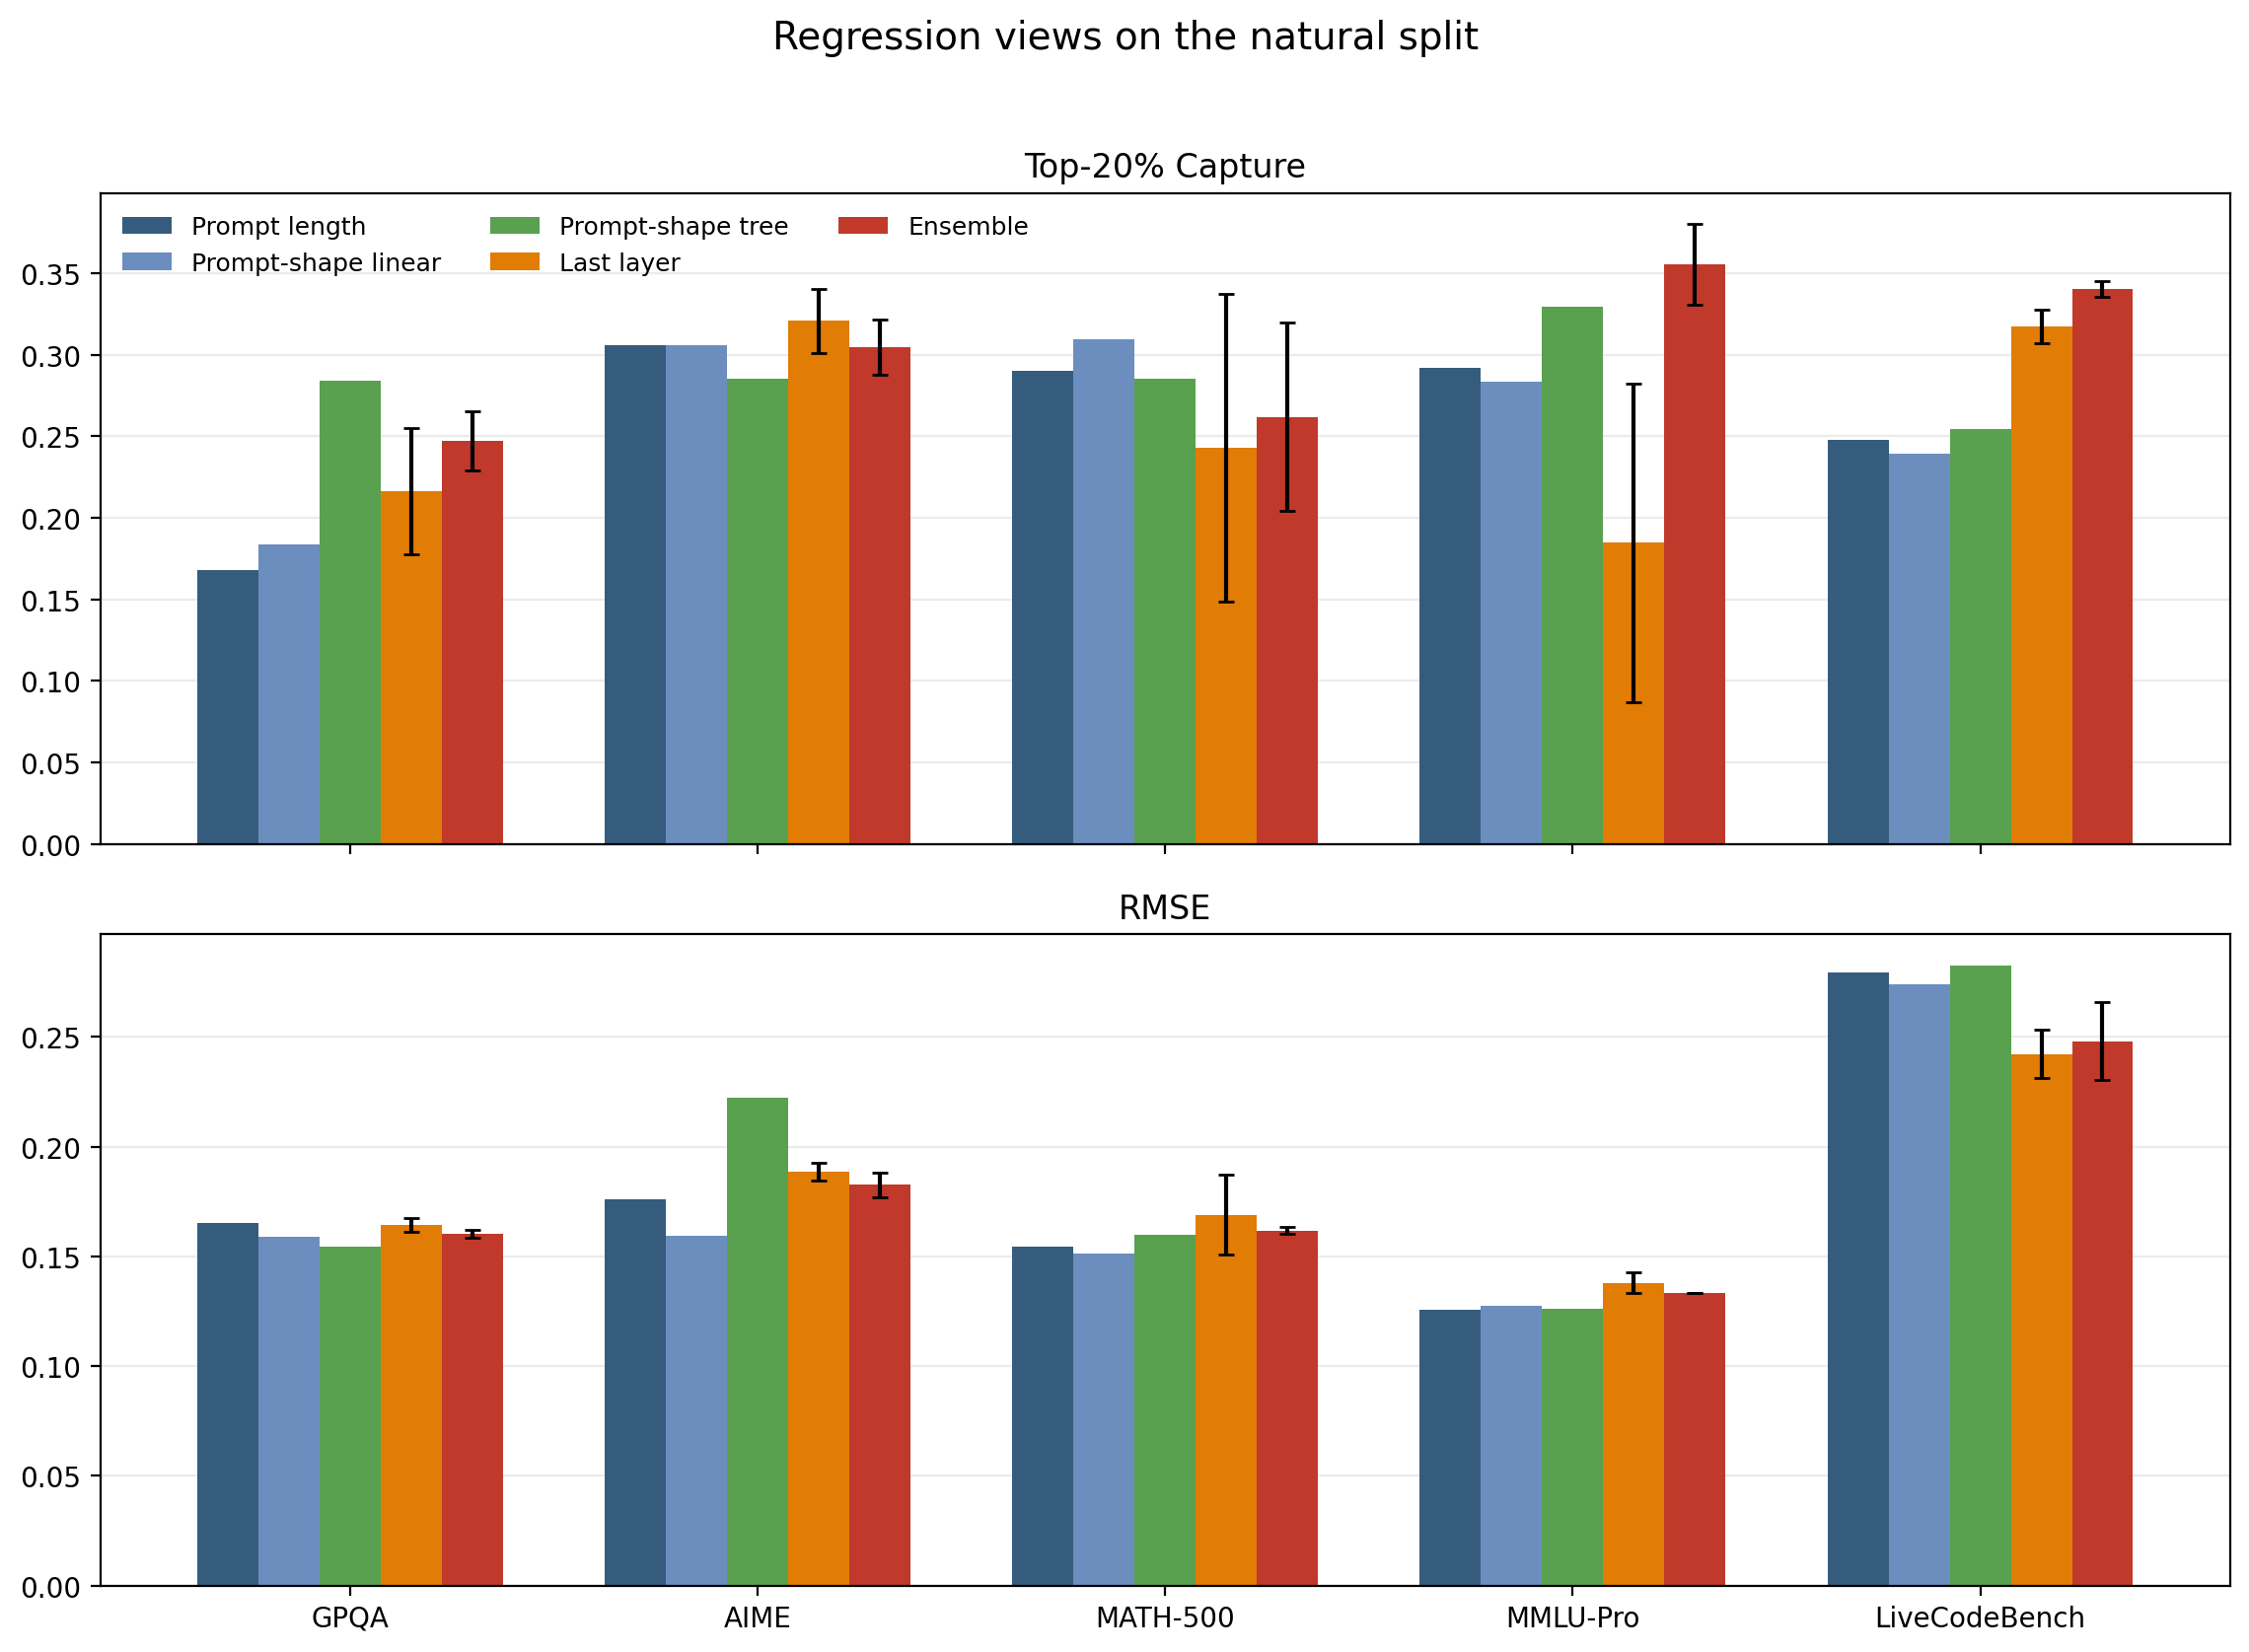
\includegraphics[width=\textwidth]{figures/regression_views.png}
\end{figure}

\begin{center}
\small
\resizebox{\textwidth}{!}{%
\begin{tabular}{@{}lrrrrrr@{}}
\toprule
Dataset & Prompt \texttt{top\_20} & Last-layer \texttt{top\_20} & Ensemble \texttt{top\_20} & Prompt \texttt{RMSE} & Last-layer \texttt{RMSE} & Ensemble \texttt{RMSE} \\
\midrule
\texttt{GPQA} & 0.168 & 0.216 +/- 0.039 & 0.247 +/- 0.018 & 0.165 & 0.164 +/- 0.003 & 0.160 +/- 0.002 \\
\texttt{AIME} & 0.306 & 0.321 +/- 0.020 & 0.305 +/- 0.017 & 0.176 & 0.189 +/- 0.004 & 0.183 +/- 0.006 \\
\texttt{MATH-500} & 0.290 & 0.243 +/- 0.094 & 0.262 +/- 0.058 & 0.154 & 0.169 +/- 0.018 & 0.162 +/- 0.002 \\
\texttt{MMLU-Pro} & 0.292 & 0.185 +/- 0.098 & 0.355 +/- 0.025 & 0.126 & 0.138 +/- 0.005 & 0.133 +/- 0.000 \\
\texttt{LiveCodeBench} & 0.248 & 0.317 +/- 0.010 & 0.340 +/- 0.005 & 0.279 & 0.242 +/- 0.011 & 0.248 +/- 0.018 \\
\bottomrule
\end{tabular}
}
\end{center}

Plain read:
\begin{itemize}[leftmargin=1.5em]
\item Screening is the right primary read for this lane.
\item Ensemble is strongest on \texttt{GPQA}, \texttt{MMLU-Pro}, and \texttt{LiveCodeBench}.
\item Prompt length still wins on calibration for \texttt{AIME}, \texttt{MATH-500}, and \texttt{MMLU-Pro}.
\item So \texttt{mean\_relative\_length} is useful as a long-completion screening score, but still mixed as a calibrated regression target.
\end{itemize}

\section*{Classification Results}
\begin{figure}[H]
\centering
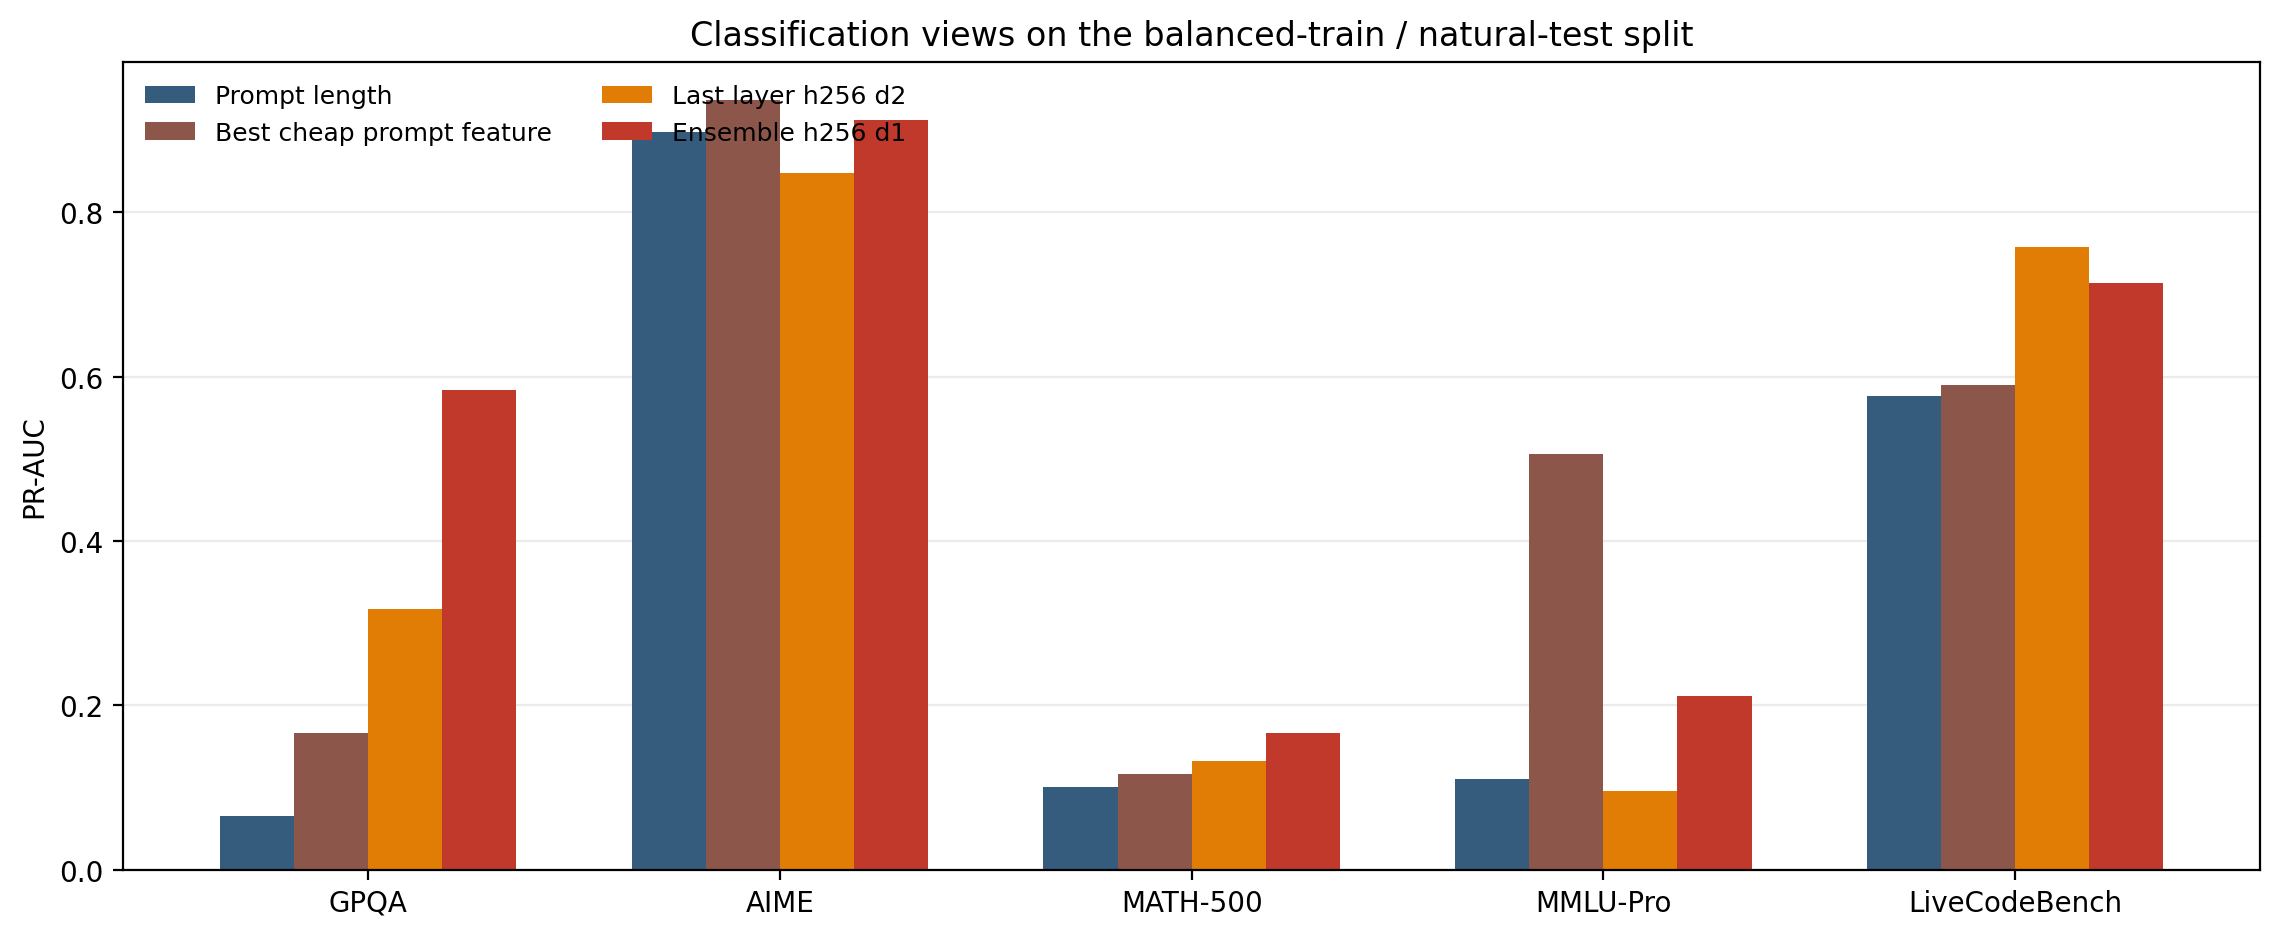
\includegraphics[width=\textwidth]{figures/binary_views.png}
\end{figure}

\begin{center}
\small
\resizebox{\textwidth}{!}{%
\begin{tabular}{@{}lrrrrrrrr@{}}
\toprule
Dataset & Prev. & Prompt \texttt{PR-AUC} & Best prompt-only & Ensemble \texttt{PR-AUC} & Prec. & Rec. & Pos. \texttt{F1} & Macro \texttt{F1} \\
\midrule
\texttt{GPQA} & 0.0500 & 0.066 & 0.167 & 0.583 & 0.214 & 1.000 & 0.345 & 0.607 \\
\texttt{AIME} & 0.5833 & 0.898 & 0.937 & 0.912 & 0.905 & 0.476 & 0.564 & 0.614 \\
\texttt{MATH-500} & 0.0400 & 0.100 & 0.117 & 0.166 & 0.054 & 0.667 & 0.100 & 0.439 \\
\texttt{MMLU-Pro} & 0.0125 & 0.110 & 0.506 & 0.212 & 0.125 & 1.000 & 0.218 & 0.575 \\
\texttt{LiveCodeBench} & 0.3375 & 0.576 & 0.590 & 0.714 & 0.614 & 0.654 & 0.514 & 0.581 \\
\bottomrule
\end{tabular}
}
\end{center}

Plain read:
\begin{itemize}[leftmargin=1.5em]
\item \texttt{majority\_s\_0.5} remains the cleaner finished head.
\item \texttt{ensemble h256 d1} is still the best single global activation surface by \texttt{PR-AUC}.
\item Threshold metrics stay recall-heavy on rare-positive datasets because train balance and test prevalence differ.
\item That is why \texttt{PR-AUC} remains the headline metric and precision / recall / \texttt{F1} stay diagnostic.
\end{itemize}

\section*{Why The Metadata Baseline Is Strong}
\begin{figure}[H]
\centering
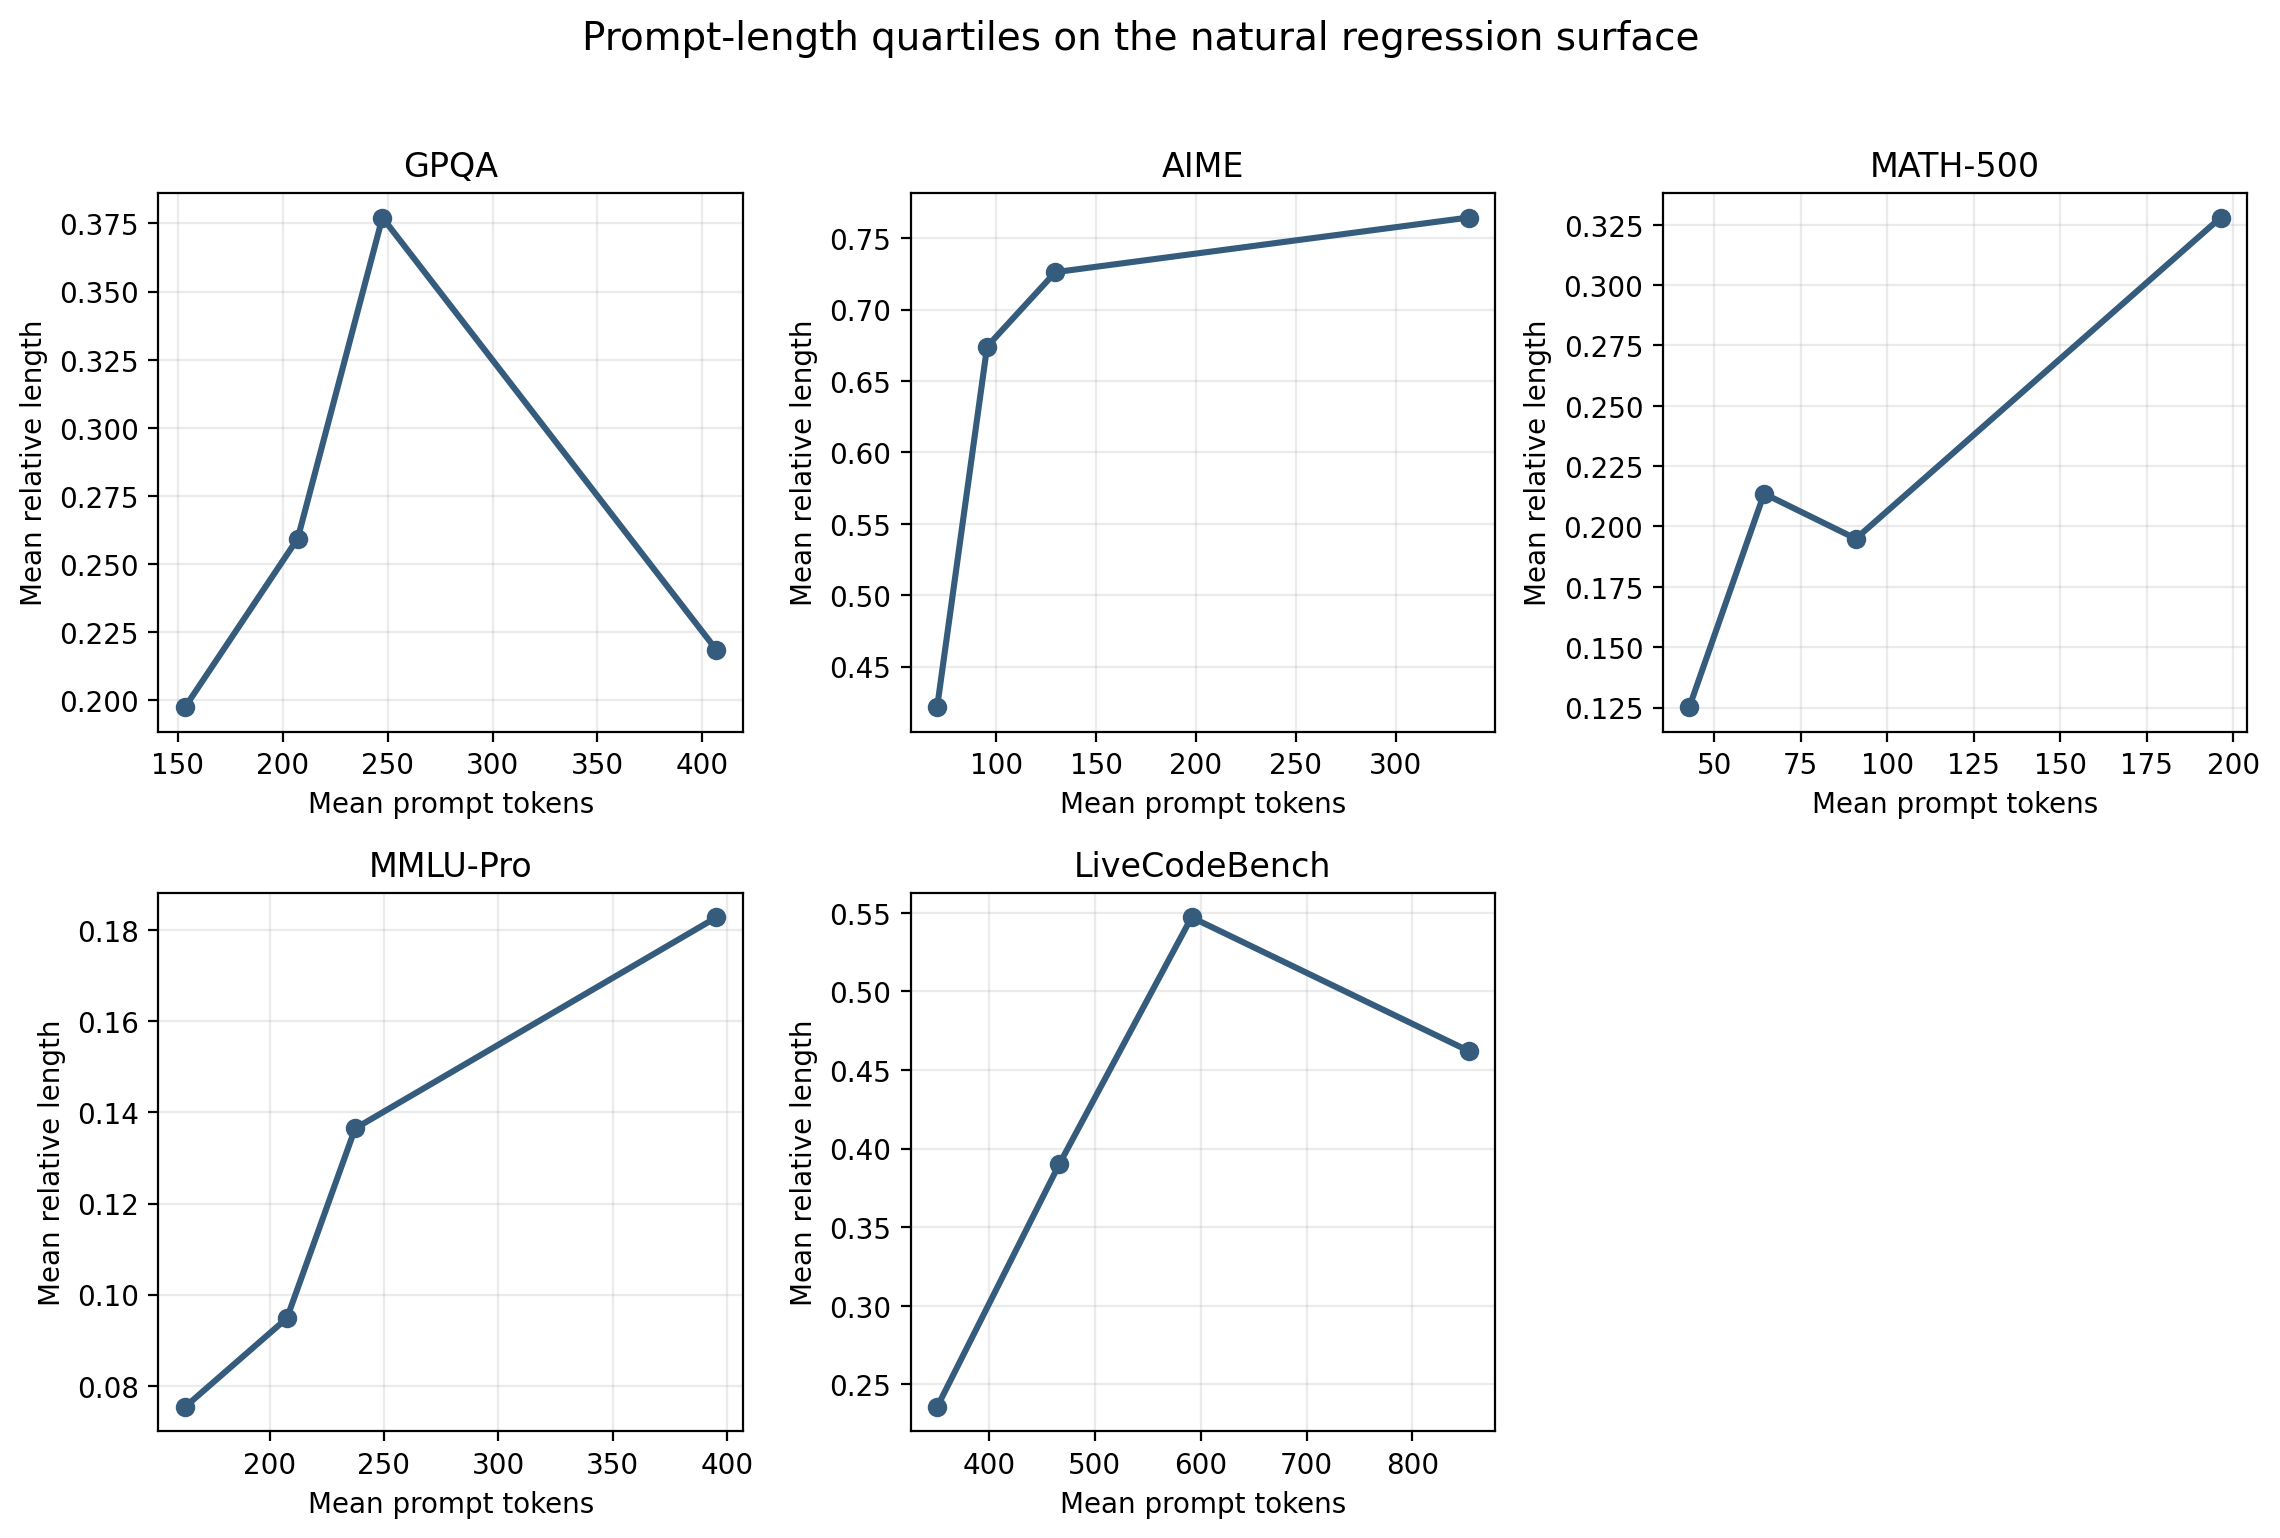
\includegraphics[width=\textwidth]{figures/prompt_length_quartiles.png}
\end{figure}

\subsection*{Prompt-only cues by dataset}
\begin{center}
\small
\begin{tabular}{@{}lp{2.2in}p{2.2in}@{}}
\toprule
Dataset & Best regression prompt-only cue & Best classification prompt-only cue \\
\midrule
\texttt{GPQA} & Newline count 0.242 & Newline count 0.167 \\
\texttt{AIME} & Character length 0.332 & Dollar count 0.937 \\
\texttt{MATH-500} & Prompt length 0.290 & Dollar count 0.117 \\
\texttt{MMLU-Pro} & Dollar count 0.300 & Newline count 0.506 \\
\texttt{LiveCodeBench} & Prompt length 0.248 & Character length 0.590 \\
\bottomrule
\end{tabular}
\end{center}

\subsection*{Plain-English interpretation}
\begin{itemize}[leftmargin=1.5em]
\item The old ``metadata baseline'' is narrow: on this run it is really just prompt length, because \texttt{effective\_max\_tokens} is fixed at \texttt{30000}.
\item Prompt length predicts completion length mostly because, on these datasets, longer prompts usually mean the prompt itself contains more work.
\item That story is strongest on \texttt{AIME}, \texttt{MATH-500}, and much of \texttt{LiveCodeBench}.
\item \texttt{MMLU-Pro} has the same effect, but more weakly.
\item \texttt{GPQA} is the honest exception: the longest prompts are not the riskiest prompts there, which is why prompt-shape models help more than raw length.
\item Classification inherits some of the same prompt-only signal because \texttt{majority\_s\_0.5} is still largely asking whether rollouts cross about half the fixed budget.
\item That is why prompt-only features can be strong on both heads without implying a hidden implementation bug.
\end{itemize}

\subsection*{Quartile read}
\begin{itemize}[leftmargin=1.5em]
\item \texttt{GPQA}: 153 -> 0.197, 207 -> 0.259, 248 -> 0.377, 407 -> 0.218
\item \texttt{AIME}: 70 -> 0.422, 96 -> 0.674, 130 -> 0.726, 336 -> 0.765
\item \texttt{MATH-500}: 43 -> 0.125, 64 -> 0.214, 91 -> 0.195, 196 -> 0.328
\item \texttt{MMLU-Pro}: 163 -> 0.075, 208 -> 0.095, 237 -> 0.137, 395 -> 0.183
\item \texttt{LiveCodeBench}: 351 -> 0.236, 467 -> 0.390, 591 -> 0.547, 853 -> 0.462
\end{itemize}

\section*{Bottom Line}
\begin{itemize}[leftmargin=1.5em]
\item Regression answer: keep the natural split / natural sampler object and read it screening-first.
\item Classification answer: keep balanced train / natural test and use \texttt{ensemble h256 d1} as the current default activation surface.
\item Metadata answer: prompt-only predictors are strong mainly because prompt surface structure already acts as a workload proxy on these fixed-budget targets.
\item Activation answer: the current surface shows lift over raw prompt length on some slices, but it still does not prove general lift over strong prompt-only controls.
\item Next honest check: a stronger prompt-shape baseline plus residualized activation lift on the natural regression head.
\end{itemize}

\section*{Artifacts}
\begin{itemize}[leftmargin=1.5em]
\item unified bundle: \texttt{outputs/prompt\_profile\_unified\_report\_20260409/}
\item source notes behind this synthesis:
  \begin{itemize}[leftmargin=1.5em]
  \item \texttt{docs/weeks/2026-W14/prompt-profile-combined-audit-2026-04-05.md}
  \item \texttt{docs/weeks/2026-W14/prompt-profile-binary-capacity-controls-2026-04-04.md}
  \item \texttt{docs/weeks/2026-W14/prompt-profile-natural-regression-rerun-2026-04-05.md}
  \item \texttt{docs/weeks/2026-W15/prompt-profile-length-mechanism-2026-04-09.md}
  \end{itemize}
\end{itemize}

\end{document}
